\chapter{Vacuum design}

\section{Pressure}

To model alpha-particle-like orbits with electrons one has to look at the number of toroidal rotations before collisions, which has to be comparable to the orbits of an alpha-particle heated device.
Therefore, the mean free path of a moving electron has to be estimated to calculate the required pressure conditions.
The mean-free path can be calculated from the temperature of the electrons $E_{kin, \beta}$ and the slowing down time $\tau$ by $l_{\beta} = \sqrt{2E_{kin, \beta}/m_{\beta}}\cdot\tau$.
For a kinetic energy of $E_{kin, \beta} \approx 200~\si{\electronvolt}$ and a slowing time of $\tau \approx \SI{10}{\milli\second}$ the resulting mean-free path $l_{\beta}$ equals to about $\SI{100}~\si{\kilo\meter}$.
In a vacuum, the electrons collide with neutrals of atomic cross-section $\sigma \approx 10^{-20}\pi ~\si{\square\meter}$ \cite{ALPS}.
Thus the required particle density $n=1/(l_{\beta}\sigma)$ is about $10^{-14}~\si{\per\cubic\meter}$.
Using the ideal gas law the required pressure conditions in the vacuum vessel are in the UHV (Ultra High Vacuum) regime $<10^{-8}~\si{\milli\bar}$.

\section{Pumps}

In order to operate a vacuum system in UHV conditions on has to consider the gas load of the system.
The gas load can be from a variety of sources, major contributions among others include initial gas contained in the system, leaks and outgassing.
At UHV conditions outgassing is the largest contributor at around $90\%$ of the total gas load \cite{outgassing}.
For metal systems the predominant residual gas species is hydrogen.
Outgassing rates can be reduced by heat treatment of the vessel and internal systems and modifying the surface of the vacuum envelope by e.g. polishing or deposition of a thin film.

The speed of a vacuum pump is defined as $S=Q/p$ with $Q=q_{p,V}$ where $Q$ is the pumping power and $p$ is the equilibrium pressure at the inlet. $q_{p,V}$ refers to the total gas load of the system at constant pressure and volume.
Pipes and hoses which connect a vacuum pump to the chamber reduce the pumping speed S at the pump to an effective vacuum speed $S_{eff}$ at the inlet to the chamber.
For practical reasons $S\approx S_{eff}$ as the vacuum pump is directly attached to the chamber.
With an estimated surface area of $\SI{15}{\square\meter}$ and an outgassing rate of $\SI{e-10}{\milli\bar\liter\per\second\per\square\cm}$ a pumping speed of about $\SI{1700}{\liter\per\second}$ at $<\SI{e-8}{\milli\bar}$ is calculated, including other gas load contributions.
This value represents just an ideal value and does not consider safety margins.
The calculations correlate with the parameters of the stellarator TJ-II \cite{vacsystj2}.

The vacuum pump of choice to achieve these conditions is a turbomolecular pump (TMP). A TMP consists of multiple stages of pairs of rotor and stator blades. The working principle is that free molecules are given a momentum in a desired direction by collisions with the blades. Gas captured in the upper stages is directed to the lower stages and compressed to the level of the fore-vacuum at the outlet side. A suitable model would be the Pfeiffer Vacuum ATH3204 MT with a DN320 ISO-F inlet flange \cite{ATH3204}, which can be seen in \ref{fig:ATH}.
The TMP is magnetically levitated, thus oil-free, and reaches a pumping speed of $\SI{3050}{\liter\per\second}$ for Nitrogen ($N_{2}$).
The maximum fore vacuum of this TMP is $\SI{3}{\milli\bar}$, therefore an adequate backing pump has to be considered, which can transport the throughput (total gas load). The maximum gas ($N_{2}$) throughput of the ATH3204 MT is $\SI{47.5}{\milli\bar\liter\per\second}$. As the total gas load at $\SI{e-8}{\milli\bar}$ is estimated at around $\SI{5e-5}{\milli\bar\liter\per\second}$ it is assumed that a backing pump with a pumping speed $S_{V}$ of about $\SI{20}{\liter\per\second}$ is sufficient. The pumping speed of the backing pump is derived from the continuity equation $Q=p_{a}\cdot S_{TMP}=p_{b}\cdot S_{V}$, where $p_{a}$ and $p_{b}$ are the respective pressures at the inlet of the TMP and backing pump. A suitable model would be the ACP 90 from Pfeiffer vacuum, an oil-free multi-stage roots pump connected via a DN 40 hose to the TMP \cite{ACP90}. At the maximum possible throughput of the TMP the chosen backing pump is not capable of transporting the gas load, therefore the use case of the two pumps has to be coordinated accordingly. During operation the TMP has to be operated according to the maximum troughput of the backing pump.

\begin{figure}[H]
    \centering
    \begin{subfigure}[b]{0.45\textwidth}
        \centering
        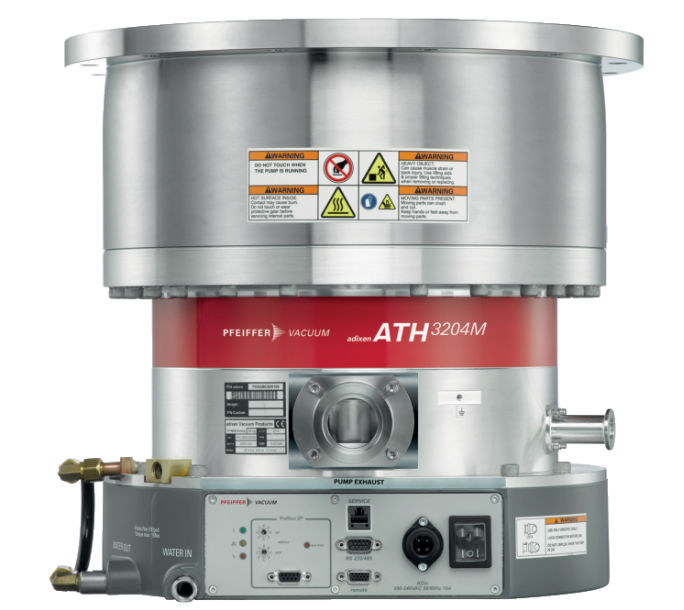
\includegraphics[width=1\textwidth]{sections/imges/vacuum_vessel/ath3204.PNG}
        \caption{Turbomolecular pump: ATH3204 MT \cite{ATH3204}.}
        \label{fig:ATH}
    \end{subfigure}
    \hfill
    \begin{subfigure}[b]{0.45\textwidth}
        \centering
        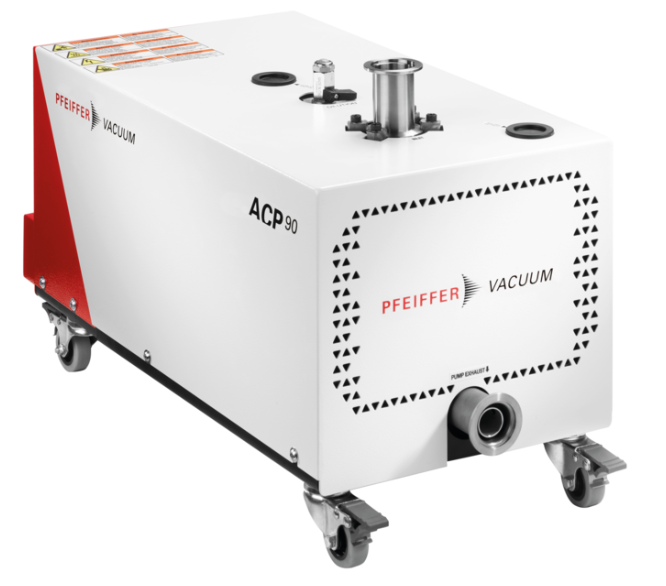
\includegraphics[width=1\textwidth]{sections/imges/vacuum_vessel/acp.PNG}
        \caption{Backing (Roughing) pump, multi-stage roots pump: ACP90 \cite{ACP90}.}
        \label{fig:ACP}
    \end{subfigure}
    \caption{Vacuum system components: (a) Turbomolecular pump and (b) Backing pump.}
    \label{fig:vacuum_system}
\end{figure}

\section{Vacuum analysis}

\subsection{Pressure measurement} \label{sec:pressure_measurement}

For the pressure measurement, a system containing a Pirani manometer for higher pressures and a Bayard-Alpert manometer for HV and UHV pressures would be suitable.
The Pirani method uses a heating wire in a tube which is connected to the vacuum to be measured.
The resistivity of the wire is temperature-dependent.
As the heat convection by the gas is pressure-dependent one can measure the change in resistivity at constant voltage to determine the pressure.
The gauge may be used for pressures between ATM and $\SI{e-4}{\milli\bar}$.
The Bayard-Alpert gauge consists of three electrodes, a hot cathode filament, a grid and an ion collector.
The filament (e.g. tungsten) emits a regulated electron current which is accelerated to the grid.
Most of the electrons collide with residual gas molecules and ionize them.
The ions are attracted by the central collector and form an ion current.
The ion current is proportional to the molecular gas pressure.
Measurement solutions like the Pfeiffer Vacuum HPT200 \cite{HPT200} and the Inficon Trigon models \cite{BCG450} are able to measure from ATM to $\SI{5e-10}{\milli\bar}$ using just one flange.

In the Fusion360 3D model, a flange was drawn for the following combination gauge, which includes both the Pirani and the Bayard-Alpert gauge \autoref{fig:Pirani_Bayard_alpert_ALL}.
All information worth knowing that guarantees the suitability of the device for the requirements at hand can be found in \autoref{fig:Pirani_technical_data}.

\begin{figure}[H]
    \centering
    \begin{subfigure}[b]{0.2\textwidth}
        \centering
        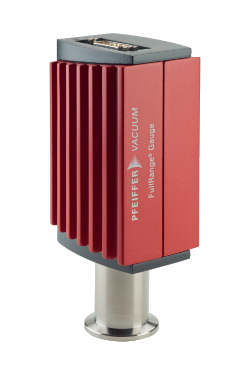
\includegraphics[width=1\textwidth]{sections/imges/vacuum_vessel/Pirani_Bayard_Alpert.PNG}
        \subcaption{}
        \label{fig:Pirani}
    \end{subfigure}
    \hfil
    \begin{subfigure}[b]{0.7\textwidth}
        \centering
        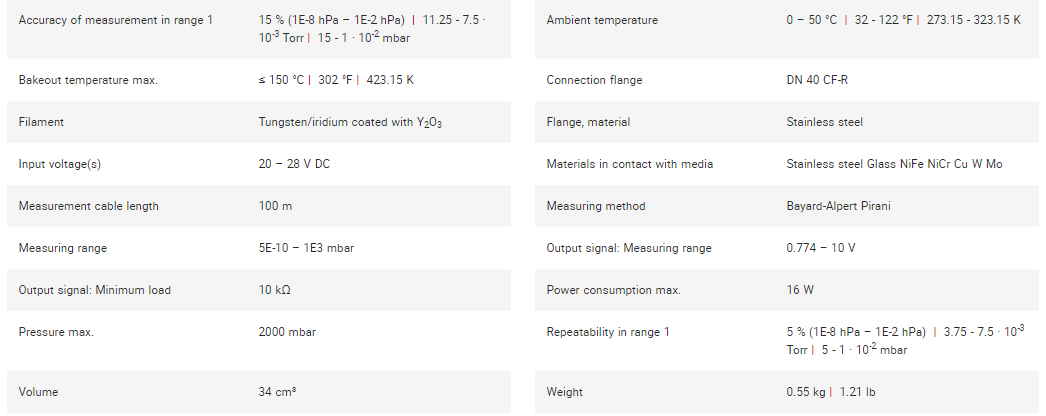
\includegraphics[width=1\textwidth]{sections/imges/vacuum_vessel/Pirani_Bayard_Alpert_technical_data.PNG}
        \subcaption{}
        \label{fig:Pirani_technical_data}
    \end{subfigure}
    \caption{Measurement device including Pirani- and Bayard-Alpert-gauge \cite{pfeifferdruck}.}
    \label{fig:Pirani_Bayard_alpert_ALL}
\end{figure}


\subsection{Residual gas analysis}

For future purposes, a mass spectrometer can be used to analyze the residual gas for the molecules it contains.
A quadrupole spectrometer was considered for this purpose \autoref{fig:Quadrupol}.
It consists of an ionizer (bombardment of molecules with electrons), an ion accelerator and a mass filter consisting of four metal rods \cite{quardrupolmassspec}.
The opposing rods are applied with the same potential consisting of an RF and a DC voltage.
The applied voltage affects the trajectory of the accelerated ions, only ions with a certain mass-to-charge ratio, which resonate, travel through the quadrupole filter to the ion detector.
A mass spectrum can be obtained by varying the applied voltage and its frequency.

\begin{figure}[H]
    \centering
    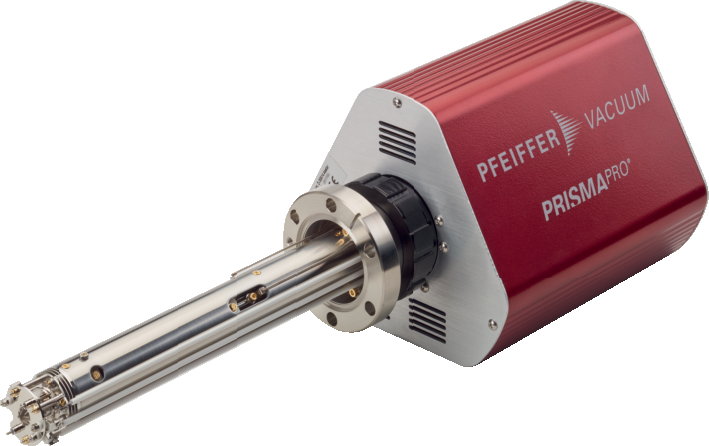
\includegraphics[width=0.6\textwidth]{sections/imges/vacuum_vessel/Quadrupol_Massenspektrometer.PNG}
    \caption{Quadrupole spectrometer: QMG 250 F1, 1-100 u, open ionsource, tungsten, I/O-option, extended \cite{pfeiffer}.}
    \label{fig:Quadrupol}
\end{figure}

There are several variants of the PrismaPro series \cite{pfeiffer}, more precisely 108 different detector designs of the quadrupole spectrometer, depending on the decision criteria pressure range, the associated necessary design, as well as the analytical performance (masses to be detected, resolution, detection limit and measuring speed).
The device features a DN40 CF-F flange and has a quadrupole length of $\SI{14.3}{\centi\meter}$.
Precision in the mass spectrometer is directly proportional to its cost.
Measurement speed influences both the signal noise and background noise.
Resolution determines the separation and signal level, with unit resolution being a common standard.
Choosing the smallest suitable mass range enhances sensitivity.
Detection limits depend on signal strength and peak overlaps, which vary based on the detector used \cite{pfeiffer}.

\section{Insulation}

As mentioned above, in UHV systems the major contributor to the total gas load is outgassing.
Outgassing of materials is temperature-dependent, thus it is key to minimize heat transfer within the UHV systems.
Insulation is key to minimize outgassing and maintaining thermal stability.
Furthermore, it plays an important role in sealing and preventing leaks, electrical insulation ensures safe operation and integrity of the system.
In UHV systems e.g. Kapton$\textsuperscript{\textregistered}$ is widely used as an insulation material for e.g. wires due to its versatility, strong dielectric properties, high-temperature resistance, low thermal outgassing and other properties.


\section{Conclusion}

For our Vacuum system a turbo-molecular pump is chosen, due to its oil-free operation and pumping speed.
It is backed up by a sufficiently sized backing pump which also provides the rough vacuum before the TMP takes over.
To reduce outgassing metal surfaces in the inside are polished and wires are heat and electrically isolated by using e.g. Kapton$\textsuperscript{\textregistered}$.
Pressure is measured using a pressure gauge that includes a Pirani device for lower vacuum levels and a Bayard-Alpert device for higher vacuum ranges.
For a residual gas analysis, one port is reserved for hosting a quadrupole mass spectrometer. The calculations for the sizing of the vacuum pumps are based on an estimated inner surface area of the vacuum system. As the outgassing rate scales with the surface area exposed to the vacuum, thus once the vacuum chamber configuration with all the components inside has been finalized, the total surface area has to be assessed. The outgassing rate per area used for the calculations is based on a typical value for UHV systems, modification might be necessary. The effective vacuum speed delivered by the vacuum pumps is highly dependent on the flow conduction through pipes and hoses. Therefore the sizing of the backing pump has to be modified depending on the length of the hose and on the use case of the TMP.


\section{Outlook}
To ensure a stable UHV enviroment, outgassing has be minimised by treatment e.g. polishing of the inner surface of the vessel. Further measures are reducing components inside the vessel, proper heat/electrical insulation of wires and leak prevention. Depending on the factors above the sizing of the TMP might have to be reconsidered. For the backing pump the effective pumping speed due to the hose has to be taking into account when choosing the size of the pump and matching of the operating modes of the TMP and backing pump.
